
\documentclass[aspectratio=169, handout]{beamer}

%\usepackage[table]{xcolor}
\mode<presentation> {
\setbeamercovered{transparent}
  \usetheme{Boadilla}

%  \usetheme{Pittsburgh}
%\usefonttheme[2]{sans}
\renewcommand{\familydefault}{cmss}
%\usepackage{lmodern}
%\usepackage[T1]{fontenc}
%\usepackage{palatino}
%\usepackage{cmbright}
\usepackage{bm}
\usepackage{listings}
\useinnertheme{rectangles}
}
\usepackage{amsmath}
\setbeamercolor{normal text}{fg=black}
\setbeamercolor{structure}{fg= blue}
\definecolor{trial}{cmyk}{1,0,0, 0}
\definecolor{trial2}{cmyk}{0.00,0,1, 0}
\definecolor{darkgreen}{rgb}{0,.4, 0.1}
\definecolor{darkpurple}{rgb}{0.4, 0, 0.6}
\usepackage{array}
\usepackage{booktabs}
\beamertemplatesolidbackgroundcolor{white}  \setbeamercolor{alerted
text}{fg=darkpurple}
\usepackage{tcolorbox}
\setbeamertemplate{caption}[numbered]\newcounter{mylastframe}

\font\domino=domino
\def\die#1{{\domino#1}}
\usepackage{tikz}
\usetikzlibrary{arrows}
\usepackage{colortbl}

\renewcommand{\familydefault}{cmss}
%\usepackage[all]{xy}

\usepackage{tikz}
\usepackage{lipsum}

 \newenvironment{changemargin}[3]{%
 \begin{list}{}{%
 \setlength{\topsep}{0pt}%
 \setlength{\leftmargin}{#1}%
 \setlength{\rightmargin}{#2}%
 \setlength{\topmargin}{#3}%
 \setlength{\listparindent}{\parindent}%
 \setlength{\itemindent}{\parindent}%
 \setlength{\parsep}{\parskip}%
 }%
\item[]}{\end{list}}
\usetikzlibrary{arrows}

\lstset{%
  language=R,
  basicstyle=\ttfamily\small,
  keywordstyle=\color{blue},
  commentstyle=\color{darkgreen},
  stringstyle=\color{darkpurple},
  showstringspaces=false,
  breaklines=true,
  frame=single,
  backgroundcolor=\color{gray!10}
}

\usecolortheme{lily}

\newtheorem{com}{Comment}
\newtheorem{lem} {Lemma}
\newtheorem{prop}{Proposition}
\newtheorem{condition}{Condition}
\newtheorem{thm}{Theorem}
\newtheorem{defn}{Definition}
\newtheorem{cor}{Corollary}
\newtheorem{obs}{Observation}
 \numberwithin{equation}{section}
 
\makeatletter
\def\beamerorig@set@color{%
  \pdfliteral{\current@color}%
  \aftergroup\reset@color
}
\def\beamerorig@reset@color{\pdfliteral{\current@color}}
\makeatother
\setbeamertemplate{navigation symbols}{}

\useoutertheme{miniframes}
\title[PLSC 30700]{Linear Models Lecture 17: Pooled and Panel Data}

\author{Robert Gulotty}
\institute[Chicago]{University of Chicago}
\vspace{0.3in}


\begin{document}



\begin{frame}
\maketitle
\end{frame}

\section{Intro}
\setcounter{subsection}{1}

\begin{frame}{From Cross-Sections to Repeated Observations}
\begin{itemize}
\item A single cross-section identifies effects only by comparing units. Adding time lets us compare a unit to itself.
\item Time can enter the model in several ways:
\begin{itemize}
\item As an indicator (before/after a policy) or as a continuous trend.
\item Through interactions, allowing slopes to vary by period (the effect of a free fedora on employment may differ today from 1940).
\end{itemize}
\item The simplest design exploits two groups at two times: \textbf{difference-in-differences}. We treat it as the on-ramp to panel data.
\end{itemize}
\end{frame}


\section{Difference in Difference}
\setcounter{subsection}{1}

\begin{frame}{Differences in Differences}
Voter ID law in Texas; Oklahoma is the control. Turnout $Y$ observed before and after.\\[4pt]
\textbf{Parameters:} $M$ = Texas baseline (e.g.\ borders Mexico), $O$ = Oklahoma baseline;\\
$T$ = common period effect (e.g.\ Trump on the ballot), $D$ = effect of the voter ID law.\pause

\vspace{6pt}
\begin{columns}[T]
\begin{column}{0.49\textwidth}
\begin{tcolorbox}[colback=blue!8, colframe=blue, title=Cross-section (after)]
\centering
\begin{tabular}{l@{\quad}l}
Texas & $M+T+D$\\
Oklahoma & $O+T$\\
\midrule
Diff & $(M-O)+D$
\end{tabular}
\end{tcolorbox}
\end{column}
\begin{column}{0.49\textwidth}
\begin{tcolorbox}[colback=darkgreen!8, colframe=darkgreen, title=Time-series (Texas)]
\centering
\begin{tabular}{l@{\quad}l}
Before & $M$\\
After & $M+T+D$\\
\midrule
Diff & $T+D$
\end{tabular}
\end{tcolorbox}
\end{column}
\end{columns}
\pause\vspace{6pt}

\centering Neither comparison alone recovers $D$.
\end{frame}


\begin{frame}{Difference-in-Differences: Recovering $D$}
Difference each state across time, then difference the within-state differences.\\[4pt]

\begin{tcolorbox}[colback=darkpurple!6, colframe=darkpurple, title=Difference-in-Differences]
\centering
\begin{tabular}{l@{\quad}ccc}
 & Before & After & After $-$ Before\\
\midrule
Texas & $M$ & $M+T+D$ & $T+D$\\
Oklahoma & $O$ & $O+T$ & $T$\\
\midrule
\multicolumn{3}{r}{Texas $-$ Oklahoma:} & $\bm{D}$\\
\end{tabular}
\end{tcolorbox}

\vspace{6pt}
\centering Within-state differences cancel $M$ and $O$; differencing them cancels $T$.
\end{frame}

\begin{frame}{Potential Outcomes}
To define the assumption that lets DD work, restate the setup formally. $D$ stays the effect size; use $G$ for the group indicator.
\begin{itemize}
\item $G\in\{0,1\}$: group indicator (1 = treated group, e.g.\ Texas; 0 = control, e.g.\ Oklahoma).
\item $t\in\{0,1\}$: period (0 = before, 1 = after).
\item $Y_t^g$: potential outcome in period $t$ if group status were $g$.
\item Observed outcome: $Y_t = G\,Y_t^1 + (1-G)\,Y_t^0$.
\item Two are observed, two are counterfactual:
\begin{itemize}
\item $Y_t^1\mid G=0$: Oklahoma's outcome had it been treated.
\item $Y_t^0\mid G=1$: Texas's outcome had it not been treated.
\end{itemize}
\item Unit-level treatment effect: $\delta_i = Y_t^1 - Y_t^0$. Across the population this averages to $D$.
\end{itemize}
\end{frame}

\begin{frame}{Parallel Trends}
DD recovers $D$ only if Texas and Oklahoma would have moved together absent the law.\\[6pt]

\begin{tcolorbox}[colback=blue!6, colframe=blue, title=Parallel trends assumption]
\centering
$$E[Y_{t=1}^0\mid G=1] - E[Y_{t=0}^0\mid G=1] \;=\; E[Y_{t=1}^0\mid G=0] - E[Y_{t=0}^0\mid G=0]$$
\end{tcolorbox}
\pause\vspace{4pt}

In the running example: $T$ enters both states the same way, and the baseline gap $M-O$ does not drift over time.\\[4pt]
\textbf{Violations:}
\begin{itemize}
\item Different state-level trends (Texas suburbanizing faster than Oklahoma).
\item Treatment-induced selection or composition change (voters moving out of Texas after the law).
\end{itemize}
\end{frame}

\begin{frame}{Parallel Trends, Visually}
\begin{center}
\includegraphics[width= 3.2 in]{DIDgraph.png}
\end{center}
\small The dotted line is the counterfactual under parallel trends: it follows the comparison group's slope. The gap on the right is the treatment effect.
\end{frame}

\begin{frame}{Obama Support: The Identification Problem}
\begin{itemize}
\item Suppose we want to study the effect of racial co-identification (non-identification) on feeling thermometers of Obama in 2008.
$$ObamaRating_i=b_0+d_O\, Black_i+\bm{b'_x}\bm{x}_i+e_i$$\pause
\item However, we are worried about the two kinds of omitted factors:
\begin{itemize}\pause
\item Time trends (T): Obama ran after a financial crisis and war that might make him popular generally.\pause
\item Group Differences (M-O): Black and white people might differ in their preferences over any president that is a relatively liberal northern antiwar Democratic senator. \pause
\end{itemize}
\item Suppose Obama's appeal (repulsion) among Black (white) people depends on the economic conditions in 2008, his being a liberal Senator, and not only his race?
\end{itemize}
\end{frame}

\begin{frame}{Obama Support: DiD with a Comparison Candidate}
\begin{itemize}
\item We can use a repeated cross section to difference out similar attitudes toward another Democratic candidate.\pause
$$Kerry_i=b_0+d_K\, Black_i+\bm{b'_x}\bm{x}_i+e_i$$
\item If we assume that
\begin{itemize}
\item All time varying factors other than the candidate's race affected Black and white people's response to Democratic nominees equally.\pause
\item All differences in evaluations of D. nominees between Black and white people did not change between the Kerry and Obama years.\pause
\end{itemize}
\item Then $\delta$ is an estimate of the Average Treatment Effect of the candidate's race on attitudes.
$$\delta=d_O-d_K=(\bar{r}_{O,B}-\bar{r}_{O,W})-(\bar{r}_{K,B}-\bar{r}_{K,W})$$
\end{itemize}
\end{frame}

\begin{frame}{Estimating Differences in Differences}
\begin{itemize}
\item Stack the Kerry and Obama waves. Define $yr08_i=1$ for 2008 survey takers and $B_i=\mathbb{I}(\text{Race="Black"})$.\pause
\item \textbf{Unrestricted} (year-specific race effect):
{\small
\begin{align*}
DRating_i=b_{0,O}\,yr08_i+b_{0,K}\,(1-yr08_i)+d_O\,yr08_i\,B_i+d_K\,(1-yr08_i)\,B_i+\bm{b'_x}\bm{x}_i+e_i
\end{align*}}\pause
\item \textbf{Restricted} ($d_O=d_K\equiv d$):
{\small
\begin{align*}
DRating_i=b_{0,O}\,yr08_i+b_{0,K}\,(1-yr08_i)+d\,B_i+\bm{b'_x}\bm{x}_i+e_i
\end{align*}}\pause
\item The F test of $H_0\!:\,d_O=d_K$ comparing the two models is the DiD test: the racial co-identification effect is $d_O-d_K$.
\end{itemize}
\end{frame}

\begin{frame}

\scriptsize{\begin{table}[!htbp] \centering 
\begin{tabular}{@{\extracolsep{5pt}}lccc} 
\\[-1.8ex]\hline 
\\[-1.8ex] & \multicolumn{3}{c}{demft} \\
\hline \\[-1.8ex] 
 I(1 - y08) & 54.5$^{***}$ & 53.0$^{***}$ &  \\ 
  & (1.4) & (1.4) &  \\ 
  & & & \\ 
y08 & 65.2$^{***}$ & 65.9$^{***}$ & 10.6$^{***}$ \\ 
  & (1.3) & (1.3) & (1.0) \\ 
  & & & \\ 
 black &  & 21.7$^{***}$ & 12.8$^{***}$ \\ 
  &  & (1.0) & (1.9) \\ 
  & & & \\ 
 I(1 - y08):black & 12.8$^{***}$ &  &  \\ 
  & (1.9) &  &  \\ 
  & & & \\ 
 y08:black & 25.1$^{***}$ &  & 12.3$^{***}$ \\ 
  & (1.2) &  & (2.3) \\ 
  & & & \\ 
   age & 0.02 & 0.02 & 0.02 \\ 
  & (0.02) & (0.02) & (0.02) \\ 
  & & & \\ 
 Constant &  &  & 54.5$^{***}$ \\ 
  &  &  & (1.4) \\ 
\hline 
\hline \\[-1.8ex] 
\end{tabular} 
\end{table} }
\end{frame}


\begin{frame}
\begin{center}
\includegraphics[width= 5 in]{ObamaDiD.png}
\end{center}
\end{frame}

\section{Panel Data}
\setcounter{subsection}{1}


\begin{frame}{From Two Cells to Many: Panel Data}
\begin{itemize}
\item DiD compared two groups at two times. Differencing cancelled time-invariant group features and group-invariant time trends.
\item Panel data observes the \emph{same} units repeatedly, so we can perform that cancellation for every unit, every period.
\item Two costs of relaxing the two-cell setup:
\begin{itemize}
\item Composition: groups must remain comparable across periods (no entry or exit driven by treatment).
\item Dependence: repeated observations on the same unit are correlated, breaking iid.
\end{itemize}
\item The remaining sections build pooled, between, and within estimators on this richer structure.
\end{itemize}
\end{frame}


\begin{frame}{Three Examples to Keep in Mind}
\begin{itemize}
\item Each pairs a time-varying outcome $Y_t$, a time-varying regressor $Z_t$, and an unobserved unit-level feature $A$ that we cannot measure directly.
\item The same machinery (within transformation, GMM moment conditions) applies to all three, but the assumptions differ.
\item As we proceed, ask of each example: which estimator handles it, and which would miss?
\end{itemize}
\end{frame}

\begin{frame}{Panel Example 1: Voting behavior}
\begin{itemize}
\item Consider a population of families.  Choose one at random.\pause
\item For each family member $t$, we observe voting decisions $Y_t$ and exposure to a persuasive messages $Z_t$.\pause
\item Each family has a household wealth $W$ and a set of stories passed down from their grandparents $A$.\pause
\item We observe $Y_t$, $Z_t$ and $W$, but not $A$. \pause
\item We want to estimate the effect of $Z_t$ on $Y_t$, holding constant $W$ and $A$.
\end{itemize}
\end{frame}

\begin{frame}{Panel Example 2: Airline cost structure}
\begin{itemize}
\item Consider a population of airlines. Choose one at random.\pause
\item In year $t$, the airline incurs cost $Y_t$ to fly $Z_t$ passengers.\pause
\item Each airline has a fixed efficiency $A$ (technology, route network, labor contracts) that does not vary over time.\pause
\item We observe $N$ randomly sampled airlines but do not measure $A$.\pause
\item Costs scale with passengers, but different airlines spend different amounts to fly the same load. We want the within-airline cost-output elasticity, separating scale economies from efficiency $A$.
\end{itemize}
\end{frame}

\begin{frame}{Panel Example 3: Candidate Electoral Performance}
\begin{itemize}
\item Consider a population of candidates. Choose one at random.\pause
\item In election cycle $t$, the candidate receives vote share $Y_t$.\pause
\item Each candidate has an underlying charisma $A$ (intrinsic appeal, base of supporters) that does not vary over time.\pause
\item We observe $N$ randomly sampled candidates across cycles, but do not measure $A$.\pause
\item Candidates with strong cycles often have strong follow-up cycles, partly because last cycle's success builds name recognition, donor networks, and incumbency benefits, and partly because they have higher charisma. We want the persistence of vote share, $Y_{t-1}\to Y_t$, separating that carryover from $A$.
\end{itemize}
\end{frame}

\begin{frame}{What These Examples Motivate}
\begin{itemize}
\item Voting in families: $A$ (grandparents' stories) likely correlates with $Z$ (messages); pooled OLS is biased and \textbf{fixed effects} restore comparability.
\item Airline costs: $A$ (proprietary technology) does not vary in time, so the \textbf{within} estimator removes it without measuring it.
\item Candidate performance: $Y_{t-1}$ appears on the right-hand side; the within transformation correlates with the error and \textbf{dynamic panel GMM} (next lecture) instruments with lagged levels.
\end{itemize}
\end{frame}


\begin{frame}{Panel Data: Terminology}
\begin{itemize}
\item The voters in a family, the airlines and candidates over time are all examples of \emph{panel data}.\pause
\item Our observations are double indexed, usually divided into $N$ units and $T$ time periods/groups. \pause
\item If there are many $T$ but few $N$, we call the data long and narrow, (time series cross section).\pause
\item If every unit is observed in every period/ group, the data are called balanced.
\end{itemize}
\end{frame}

\begin{frame}{Greene's Airline Panel}
\begin{itemize}
\item Greene analyzes the cost structure in the airline industry from 1970-84.
\item Research question: do airlines have positive economies of scale?
\item library(AER); data("USAirlines"); analyzes determinants of total costs for 6 airlines.\pause
\item The cost function follows a Cobb-Douglas specification. Taking logs yields a linear regression:
$$\ln(\text{cost})= \beta_0+\beta_1\ln(\text{output})+\beta_2\ln(\text{fuel price})+\beta_3\text{load}+u$$
\item \emph{cost}: total costs of labor materials etc in USD 1000.
\item \emph{output}: revenue passenger mile index
\item input \emph{prices}: fuel prices
\item \emph{load}: share of seats sold on flights flown.
\end{itemize}
\end{frame}


\section{Pooled Data}
\setcounter{subsection}{1}



\begin{frame}{Airline Panel: Six Carriers, 15 Years}
\begin{center}
\includegraphics[width= 4.5 in]{airpanel.png}
\end{center}
\small Log total cost, 1970--1984. Levels differ across carriers; all rise together over time.
\end{frame}



\begin{frame}{Pooled Regression of log(costs)}
\begin{table}
\begin{center}
\begin{tabular}{l c c}
\hline
 & Greene 2000& Greene 2003 \\
\hline
(Intercept)  & $9.52^{***}$  & $9.42^{***}$  \\
             & $(0.23)$      & $(0.23)$      \\
lnoutput     & $0.88^{***}$  & $0.94^{***}$  \\
             & $(0.01)$      & $(0.03)$      \\
lnpfuel      & $0.45^{***}$  & $0.46^{***}$  \\
             & $(0.02)$      & $(0.02)$      \\
load         & $-1.63^{***}$ & $-1.54^{***}$ \\
             & $(0.35)$      & $(0.34)$      \\
lnoutput$^2$ &               & $0.02^{*}$    \\
             &               & $(0.01)$      \\
\hline
R$^2$        & $0.99$        & $0.99$        \\
Num. obs.    & $90$          & $90$          \\
\hline
\end{tabular}
\end{center}
\end{table}
\end{frame}

\begin{frame}{Where Does the Variation Come From?}
\begin{itemize}
\item Before reading off pooled coefficients, look at the data the way pooled OLS does: every airline-year is one point.
\item Then strip off the airline-specific mean and ask what is left within an airline.
\item The next plots compare those views for output, fuel price, and load.
\end{itemize}
\end{frame}

\begin{frame}{Cost and Output: Raw Scatter}
\begin{center}
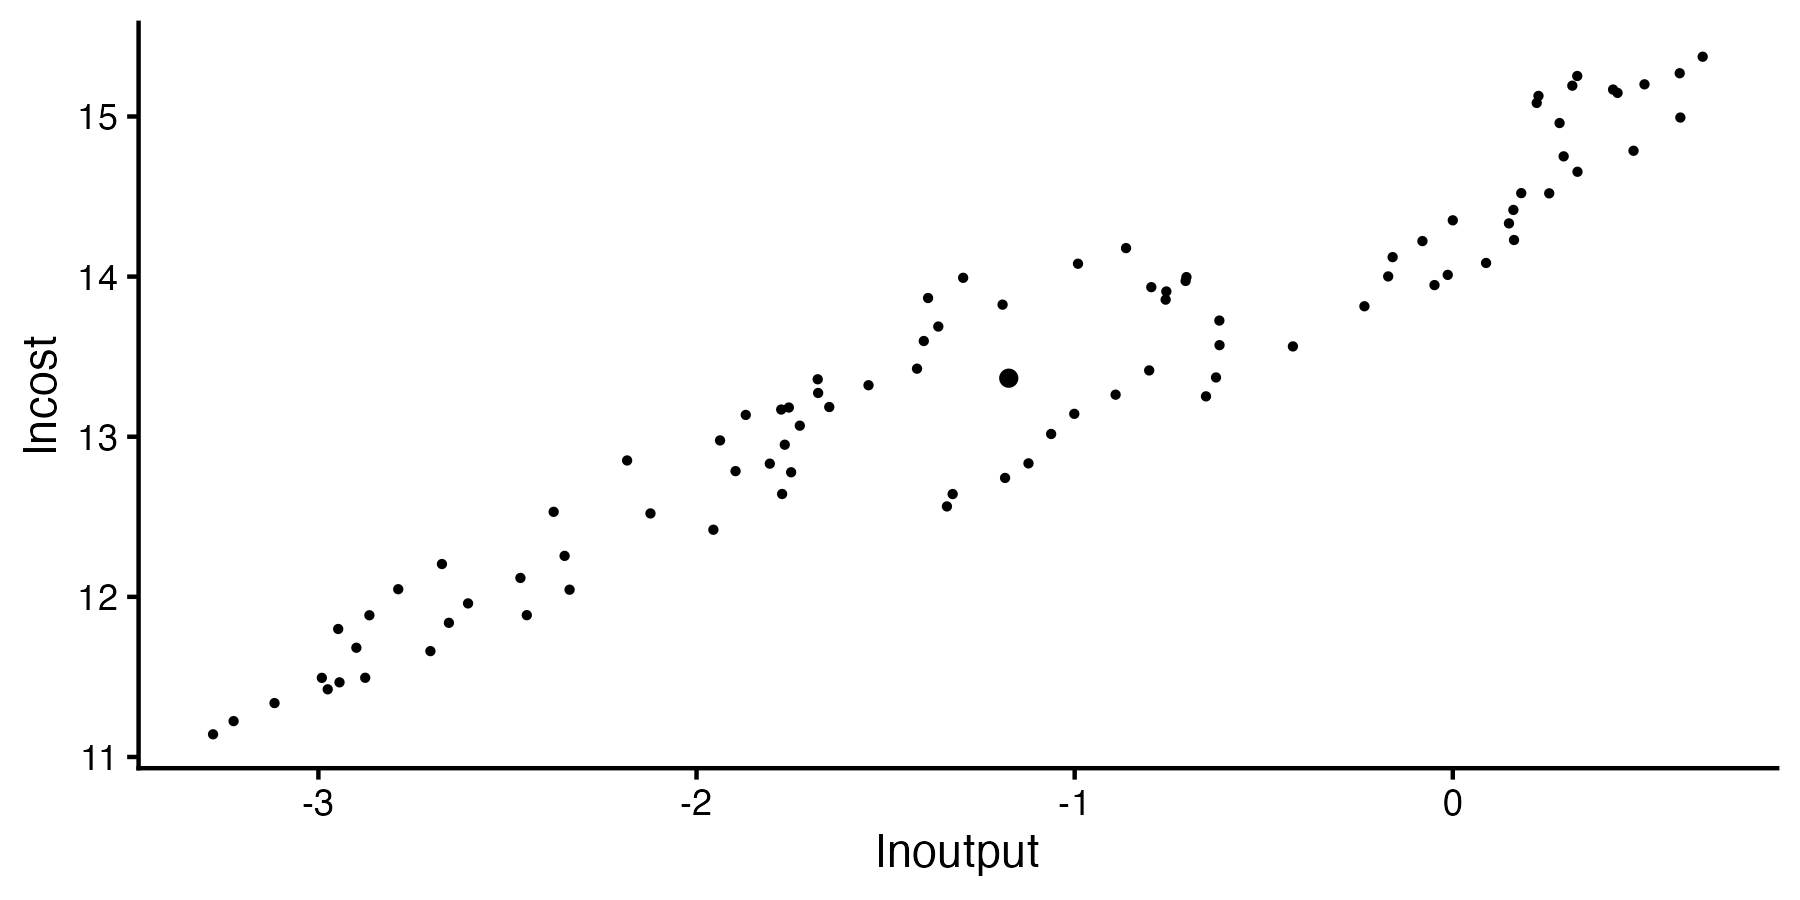
\includegraphics[width= 4.3 in]{airgrandmean0.png}
\end{center}
\small 90 airline-years pooled. The black dot is the grand mean $(\overline{\overline{\text{lnoutput}}},\,\overline{\overline{\text{lncost}}})$, the only summary a single OLS fit will use.
\end{frame}

\begin{frame}{Cost and Output: Pooled, Between, Within}
\begin{center}
\includegraphics[width= 4.3 in]{airgrandmean.png}
\end{center}
\small Coloured lines: each airline through time (within variation). Large coloured dots: airline means (between variation). Black line: pooled OLS fit.
\end{frame}


\begin{frame}{Cost and Fuel Price}
\begin{center}
\includegraphics[width= 4.3 in]{airgrandmean2.png}
\end{center}
\small Within and between move the same way (prices rose over the 1970s for everyone), so the pooled slope is close to the within slope.
\end{frame}

\begin{frame}{Cost and Capacity Utilization (load)}
\begin{center}
\includegraphics[width= 4.3 in]{airgrandmean3.png}
\end{center}
\small Bivariate pooled slope is mildly \emph{positive}: airlines that run fuller planes also have higher total costs, because larger carriers do both.
\end{frame}

\begin{frame}{Cost and Load, partialling out output and fuel price}
\begin{center}
\includegraphics[width= 4.3 in]{airgrandmean4.png}
\end{center}
\small Residual scatter from regressing both variables on $(\text{lnoutput},\text{lnpfuel})$. Slope flips to $-1.63$: holding scale and input prices fixed, fuller planes are cheaper.
\end{frame}

\begin{frame}{What the Plots Show}
\begin{itemize}
\item For output and fuel price, within and between push the same way, so pooled OLS looks fine.
\item For load, between-airline variation reverses the sign relative to within. The bivariate pooled scatter is misleading.
\item Partialling out the other regressors recovers the within-airline relationship. FE will do this for all variables at once.
\end{itemize}
\end{frame}


\begin{frame}{Three Flavors of Exogeneity in Panel Data}
Each panel estimator needs a different version of ``$\bm{x}$ uncorrelated with $\bm{e}$'' across time. Listed weakest to strongest:\\[4pt]

\centering
\small
\begin{tabular}{@{}p{3.3cm}p{5.6cm}p{4.6cm}@{}}
\toprule
\textbf{Assumption} & \textbf{Formal statement} & \textbf{Used by} \\
\midrule
Contemporaneous & $E[e_{it}\mid\bm{x}_{it}]=0$ & Pooled OLS \\
 & (plus $\alpha_i$ uncorrelated with $\bm{x}_{it}$, else FE) & \\[6pt]
Sequential (predetermined) & $E[e_{it}\mid\bm{x}_{i1},\ldots,\bm{x}_{it}]=0$ & Arellano-Bond (next lecture) \\
 & feedback $e_{it}\to\bm{x}_{i,t+1}$ allowed & with lagged $Y$ as a regressor\\[6pt]
Strict & $E[e_{it}\mid\bm{x}_{i1},\ldots,\bm{x}_{iT}]=0$ for all $t$ & Within (FE), Between \\
 & no feedback, no anticipation & \\
\bottomrule
\end{tabular}

\vspace{8pt}
\flushleft
\textbf{What violates strict exogeneity.} Lagged dependent variables on the right-hand side, feedback from $Y$ to future $X$, anticipation of future treatment, time-varying confounders.
\end{frame}

\begin{frame}{Autocorrelation versus Autoregression}
\begin{align*}
Y_t&=\alpha Y_{t-1}+\beta X_t+\nu_t\\
\nu_t&=\rho \nu_{t-1}+e_t
\end{align*}
\begin{itemize}\pause
\item $\rho\neq 0$, $\alpha = 0$ has a "common factor" problem (autocorrelation): 
\begin{itemize}
\item Outcomes at $t-1$ are associated with outcomes at $t$ for many unobserved reasons.
\item OLS slope estimates are unbiased but inefficient and produces wrong standard errors.
\item Addressed with GLS/ serial correlation robust standard errors. \pause
\end{itemize}
\item $\alpha \neq 0$ is associated with dynamics: 
\begin{itemize}
\item Outcomes at $t-1$ affect outcomes now.
\item OLS is biased, inefficient and produces wrong standard errors. 
\item Addressed with lagged variables and other structural time series approaches.
\end{itemize}
\end{itemize}
\end{frame}


\begin{frame}{Improvements on Inference}
\begin{itemize}
\item In panel data we likely violate of iid errors, as observations from the same group/firm are likely associated
$$E[e_{ig}e_{jg}]=\rho\sigma^2_e>0 $$
\item Here $\rho$ is the intra-group/firm correlation.
\end{itemize}
\end{frame}
%
%\begin{frame}{How far off are we?}
%\begin{itemize}
%\item Consider an additive model of the residuals.
%$$e_{ig}=\nu_g+\eta_{ig}$$\pause
%\item Where $v_g$ is a random shock for group g, and $\eta_{ig}$ is the remaining individual level component.\pause
%\item Given this error structure: $\rho=\frac{\sigma^2_\nu}{\sigma^2_\nu+\sigma^2_\eta}$\pause
%\item With the same sample sizes across time,
%$$\frac{V(\hat{\beta}_1)}{V_{regular}(\hat{\beta}_1)}=1+(n-1)\rho$$\pause
%\item If $\rho=1$, then $V_{regular}(\hat{\beta}_1)$ should be $n$ times larger!
%\end{itemize}
%\end{frame}


\begin{frame}{Standard error problems.}
\begin{itemize}
\item If the number of groups is large, we can cluster standard errors using a formula similar to White standard errors.\pause
\item If the number of groups is small, we can just inflate our standard errors by $\sqrt{1+(n_g-1)\rho}$ (the Moulton factor; $n_g$ is the (average) cluster size).\pause
\item There is a bootstrap solution that has good performance
\end{itemize}
\end{frame}


\begin{frame}{White vs Cluster Robust}
\begin{table}
\begin{center}
\begin{tabular}{l c c}
\hline
 & (white) & (cluster by airline) \\
\hline
(Intercept) & $9.52^{***}$  & $9.52^{***}$ \\
            & $(0.22)$      & $(0.38)$     \\
lnoutput    & $0.88^{***}$  & $0.88^{***}$ \\
            & $(0.01)$      & $(0.02)$     \\
lnpfuel     & $0.45^{***}$  & $0.45^{***}$ \\
            & $(0.02)$      & $(0.03)$     \\
load        & $-1.63^{***}$ & $-1.63^{*}$  \\
            & $(0.32)$      & $(0.44)$     \\
\hline
R$^2$       & $0.99$        & $0.99$       \\
N Clusters  & $$            & $6$          \\
\hline
\end{tabular}
\end{center}
\end{table}
\end{frame}

\section{Between and Within Estimators}
\setcounter{subsection}{1}

\begin{frame}{From Fixing Inference to Using the Panel Structure}
\begin{itemize}
\item Clustered SEs adjust the variance of $\hat{\bm{b}}_P$ but leave the coefficient alone.
\item The deeper problem is bias when $\alpha_i$ is correlated with $\bm{X}_{it}$: pooled OLS averages it in.\pause
\item Each unit is observed $T$ times. Differencing each variable from its own unit mean cancels $\alpha_i$ without ever observing it.
\item That move defines the within (fixed-effects) estimator. We derive it next, then show that pooled OLS is itself a weighted average of within and between.
\end{itemize}
\end{frame}

\begin{frame}{Fixed Effects: Two Equivalent Approaches}
Panel model $y_{it}=\bm{\beta}'\bm{x}_{it}+\alpha_i+e_{it}$, with $E[e_{it}\mid\alpha_i,\bm{x}_{i\cdot}]=0$ but $E[\alpha_i\mid\bm{x}_{it}]\neq 0$ (so pooled OLS is biased).\\[6pt]

\begin{columns}[T]
\begin{column}{0.48\textwidth}
\begin{tcolorbox}[colback=blue!8, colframe=blue, title=Dummy variables]
Add one dummy per unit, run OLS:
$$\bm{y}=\bm{X}\bm{\beta}+\bm{D}\bm{\alpha}+\bm{e}.$$
The $N$ fitted dummies absorb the unit intercepts.
\end{tcolorbox}
\end{column}
\begin{column}{0.48\textwidth}
\begin{tcolorbox}[colback=darkgreen!8, colframe=darkgreen, title={Demean within units, then regress}]
Subtract each variable's own unit mean and run OLS:
$$y_{it}-\bar{y}_i=\bm{\beta}'(\bm{x}_{it}-\bar{\bm{x}}_i)+\tilde e_{it}.$$
The $\alpha_i$ cancels because $\alpha_i-\bar\alpha_i=0$.
\end{tcolorbox}
\end{column}
\end{columns}
\vspace{4pt}

\textbf{Both produce the same $\hat{\bm{\beta}}$.} Why: Frisch-Waugh-Lovell turns the dummy regression into a regression on within-demeaned variables. The next three slides prove it.
\end{frame}

\begin{frame}{Why the Two Match: Frisch-Waugh-Lovell}
By FWL, the slope on $\bm{X}$ in the dummy regression equals OLS run on $\bm{X}$ and $\bm{y}$ after partialling $\bm{D}$ out of both:
$$\hat{\bm{\beta}}=(\bm{X}'\bm{M}_D\bm{X})^{-1}\bm{X}'\bm{M}_D\bm{y}, \qquad \bm{M}_D=\bm{I}-\bm{D}(\bm{D}'\bm{D})^{-1}\bm{D}'.$$
$\bm{M}_D$ is the residual maker for the dummy regression: $\bm{M}_D\bm{v}$ is whatever is left of $\bm{v}$ after a regression on the unit dummies alone.\\[6pt]

\textbf{Claim.} For any variable $\bm{v}$, $\bm{M}_D\bm{v}$ is $\bm{v}$ minus its unit mean: $(\bm{M}_D\bm{v})_{it}=v_{it}-\bar{v}_i$. Granted the claim, the dummy estimator runs OLS on the within-demeaned data. The next two slides verify the claim for $N=2$.
\end{frame}

\begin{frame}{Computing $\bm{M}_D$ for $N=2$}
\begin{itemize}
\item $\bm{D}=\begin{pmatrix} \bm{i}&\bm{0}\\\bm{0}&\bm{i}\end{pmatrix}$ where $\bm{i}$ is a ($T\times 1$) vector of 1s.\pause
\begin{align*}
\bm{M}_D&=\bm{I}-\bm{D}(\bm{D}'\bm{D})^{-1}\bm{D}'\\\pause
&=\begin{pmatrix} \bm{I}&\bm{0}\\\bm{0}&\bm{I}\end{pmatrix}-\begin{pmatrix} \bm{i}&\bm{0}\\\bm{0}&\bm{i}\end{pmatrix}\left[\begin{pmatrix} \bm{i}'&\bm{0}\\\bm{0}&\bm{i}'\end{pmatrix}\begin{pmatrix} \bm{i}&\bm{0}\\\bm{0}&\bm{i}\end{pmatrix}\right]^{-1}\begin{pmatrix} \bm{i}'&\bm{0}\\\bm{0}&\bm{i}'\end{pmatrix}\\\pause
&=\begin{pmatrix} \bm{I}&\bm{0}\\\bm{0}&\bm{I}\end{pmatrix}-\begin{pmatrix} \bm{i}&\bm{0}\\\bm{0}&\bm{i}\end{pmatrix}\begin{pmatrix}T&\bm{0}\\\bm{0}&T\end{pmatrix}^{-1}\begin{pmatrix} \bm{i}'&\bm{0}\\\bm{0}&\bm{i}'\end{pmatrix}\\\pause
&=\begin{pmatrix} \bm{I}&\bm{0}\\\bm{0}&\bm{I}\end{pmatrix}-\begin{pmatrix} \bm{i}&\bm{0}\\\bm{0}&\bm{i}\end{pmatrix}\begin{pmatrix} 1/T&\bm{0}\\\bm{0}&1/T\end{pmatrix}\begin{pmatrix} \bm{i}'&\bm{0}\\\bm{0}&\bm{i}'\end{pmatrix}\\\pause
&=\begin{pmatrix} \bm{I}-\frac{1}{T}\bm{i}\bm{i}'&\bm{0}\\\bm{0}&\bm{I}-\frac{1}{T}\bm{i}\bm{i}'\end{pmatrix}
\end{align*}\pause 
\end{itemize}
\end{frame}



\begin{frame}{$\bm{M}_D\bm{y}$ Is the Within-Demeaned Vector}
Writing $\bar{y}_i = \frac{1}{T}\sum_t y_{it}$ for unit $i$'s mean:
\begin{align*}
\bm{M}_D\bm{y}&=\begin{pmatrix} \bm{I}-\frac{1}{T}\bm{i}\bm{i}'&\bm{0}\\\bm{0}&\bm{I}-\frac{1}{T}\bm{i}\bm{i}'\end{pmatrix}\begin{pmatrix}\bm{y}_1\\ \bm{y}_2 \end{pmatrix}
=\begin{pmatrix}
y_{11}-\bar{y}_1\\
\vdots\\
y_{1T}-\bar{y}_1\\
y_{21}-\bar{y}_2\\
\vdots\\
y_{2T}-\bar{y}_2
\end{pmatrix}.
\end{align*}
The $i$th block of $\bm{M}_D\bm{y}$ is $\bm{y}_i$ with unit $i$'s own mean subtracted. The same operation applied column-by-column to $\bm{X}$ gives $\bm{M}_D\bm{X}$. Equivalence to the dummy regression is now confirmed.
\end{frame}

\begin{frame}{The Within Estimator: Closed Form and Computation}
Equivalence confirmed: $\bm{M}_D\bm{X}$ and $\bm{M}_D\bm{y}$ are the within-demeaned data, so the FE slope is OLS on those demeaned variables:
$$\hat{\bm{\beta}}_W=(\bm{S}_{xx}^W)^{-1}\bm{S}_{xy}^W,$$
$$\bm{S}_{xx}^W=\sum_{i,t}(\bm{x}_{it}-\bar{\bm{x}}_i)(\bm{x}_{it}-\bar{\bm{x}}_i)',\qquad \bm{S}_{xy}^W=\sum_{i,t}(\bm{x}_{it}-\bar{\bm{x}}_i)(y_{it}-\bar{y}_i).$$
\vspace{2pt}

\textbf{In practice.} Demean every variable by its unit mean and run OLS. The residual degrees of freedom shrink from $NT-k$ to $NT-N-k$ to account for the $N$ estimated unit means.
\end{frame}




\begin{frame}{Stacked Matrix Notation}
$\bm{y}_i$: $T\times 1$, $\bm{X}_i$:  $T\times k$, $\bm{e}_i$: $T\times 1$, $\bm{\beta}:$ $k\times 1$
\pause
\begin{align*}
\begin{bmatrix}\bm{y}_1\\\bm{y}_2\\ \vdots \\ \bm{y}_N \end{bmatrix}&=\begin{bmatrix}\bm{X}_1\\\bm{X}_2\\ \vdots \\ \bm{X}_N \end{bmatrix} \bm{\beta}+\begin{bmatrix}\alpha_1 \bm{1}\\\alpha_2 \bm{1}\\ \vdots \\ \alpha_N \bm{1} \end{bmatrix}+\begin{bmatrix}\bm{e}_1\\\bm{e}_2\\ \vdots \\ \bm{e}_N \end{bmatrix}\\\pause
y&= \bm{X}\bm{\beta}+\bm{\alpha}\otimes \bm{1}_T+\bm{e}
\end{align*}
\end{frame}


\begin{frame}{Software Implementations}
\begin{itemize}
\item lm(y$\sim x+f_1+f_2+\ldots +f_n)$
\item plm(y$\sim x$, c("unit", "time")
\item fixest::feols(y$\sim$ x$|$ fe)
\item You can also demean by time averages, but you need to correct the standard errors.
\end{itemize}
\end{frame}


\begin{frame}{Why Demeaning Removes the Unit Effect}
The FE model writes
$$y_{it}=\bm{\beta}'\bm{x}_{it}+\alpha_i+e_{it}.$$
Subtract each variable's unit mean:
$$y_{it}-\bar{y}_i=\bm{\beta}'(\bm{x}_{it}-\bar{\bm{x}}_i)+(\alpha_i-\bar{\alpha}_i)+(e_{it}-\bar{e}_i).$$
\textbf{Key step.} Since $\alpha_i$ does not vary in $t$,
$$\bar{\alpha}_i = \tfrac{1}{T}\sum_{t=1}^T \alpha_i = \alpha_i, \qquad \text{so}\qquad \alpha_i-\bar{\alpha}_i = 0.$$
The unit effect drops out of the demeaned equation. Demeaning removes $\alpha_i$ without our ever observing or estimating it.\\[4pt]
What remains, $\tilde y_{it}=\bm{\beta}'\tilde{\bm{x}}_{it}+\tilde e_{it}$, is what OLS on the demeaned data fits.
\end{frame}



\begin{frame}{Cost and Output: Pooled Fit}
\begin{center}
\includegraphics[width= 4.3 in]{airgrandmean.png}
\end{center}
\small Single black line: pooled OLS slope $\hat\beta=0.88$, averaging across and within airlines.
\end{frame}

\begin{frame}{Cost and Output: Within Fit}
\begin{center}
\includegraphics[width= 4.3 in]{airgrandmeanFe.png}
\end{center}
\small Per-airline fits with a common slope but separate intercepts. Within slope $\hat\beta=0.92$ is steeper than pooled because the flatter between-airline relationship pulls the pooled line down.
\end{frame}

\begin{frame}{Small note on estimation}
$$\bm{b}_{fe}=\bm{\beta}+(\bm{X}'\bm{M}_D\bm{X})^{-1}\bm{X}'\bm{M}_D\bm{e}$$
Under iid errors, we have:
$var(\bm{b}_{fe})=\sigma_{e}^2(\bm{X}'\bm{M}_D\bm{X})^{-1}$.
But we need to correct our estimator for the $N$ estimated means:
$$s_e^2=\frac{\sum_{i=1}^N\sum_{t=1}^T e^2_{it}}{NT-N-K}$$
\end{frame}

\begin{frame}{Fixed Effects as GMM Moment Conditions}
\begin{itemize}
\item Define the within-transformed variables $\tilde{Y}_{it}=Y_{it}-\bar{Y}_i$ and $\tilde{\bm{X}}_{it}=\bm{X}_{it}-\bar{\bm{X}}_i$.
\item The FE (within) estimator solves the moment conditions:
$$E[\tilde{\bm{X}}_{it}'\tilde{e}_{it}]=\bm{0}$$\pause
\item This is a \textbf{just-identified} GMM problem: $k$ moment conditions for $k$ parameters.
\begin{itemize}
\item No overidentifying restrictions $\Rightarrow$ no $J$-test with FE alone.
\end{itemize}\pause
\item \textbf{Preview:}
\begin{itemize}
\item Random effects adds between-group moments $\Rightarrow$ more efficient under stronger assumptions.
\item Arellano-Bond (next lecture) creates \emph{many} moment conditions from lagged levels $\Rightarrow$ overidentification $\Rightarrow$ testable with $J$-statistic.
\end{itemize}
\end{itemize}
\end{frame}

\begin{frame}{Pooled Regression Anatomy}
\small Rewrite pooled OLS in the notation we will reuse for between and within.\\[2pt]
\begin{itemize}
\item Let $\bm{x}_{it}$ be the $k\times 1$ vector of regressors. Grand means: $\bm{\bar{\bar{x}}}\equiv \frac{1}{NT}\sum_{i,t} \bm{x}_{it}$, $\bar{\bar{y}}\equiv \frac{1}{NT}\sum_{i,t} y_{it}$.\pause
\item The pooled estimator: $\bm{b_P}=(\bm{S}^P_{xx})^{-1}\bm{S}_{xy}^P$ with
$$\bm{S}^P_{xx}= \sum_{i,t}(\bm{x}_{it}-\bar{\bar{\bm{x}}})(\bm{x}_{it}-\bar{\bar{\bm{x}}})',\qquad \bm{S}^P_{xy}= \sum_{i,t}(\bm{x}_{it}-\bar{\bar{\bm{x}}})(y_{it}-\bar{\bar{y}}).$$
\end{itemize}
\end{frame}

\begin{frame}[fragile]
  \begin{lstlisting}
airlines<-airlines%>% mutate(
  mlnoutput = mean(lnoutput),
  mlnpfuel = mean(lnpfuel),
  mload = mean(load))
    
Xp<-airlines%>%transmute(
		lnoutputdm = lnoutput-mlnoutput, 
		lnpfueldm = lnpfuel-mlnpfuel,
		loaddm = load-mload)%>%
		as.matrix()

Sp_xx = t(Xp)%*%Xp
  \end{lstlisting}
\end{frame}



\begin{frame}{Between Regression}
Within threw away all cross-unit variation; \textbf{between} does the opposite: it uses only cross-unit variation.\\[4pt]
\textbf{Construction.} Collapse each unit's $T$ observations into one point at its means; run OLS on the resulting $N$-observation cross section:
$$\bar{y}_i=\bm{\beta}'\bar{\bm{x}}_i+\bar{e}_i, \qquad i=1,\ldots,N.$$
The slope is $\bm{b}_B=(\bm{S}^B_{xx})^{-1}\bm{S}^B_{xy}$ with
$$\bm{S}^B_{xx} = \sum_{i=1}^N T\,(\bar{\bm{x}}_i-\bar{\bar{\bm{x}}})(\bar{\bm{x}}_i-\bar{\bar{\bm{x}}})',\qquad \bm{S}^B_{xy} = \sum_{i=1}^N T\,(\bar{\bm{x}}_i-\bar{\bar{\bm{x}}})(\bar{y}_i-\bar{\bar{y}}).$$
The factor of $T$ keeps these sums on the same scale as $\bm{S}^P$ and $\bm{S}^W$, so $\bm{S}^P=\bm{S}^B+\bm{S}^W$ on the next slide.
\end{frame}

\begin{frame}[fragile]
  \begin{lstlisting}
airlines<-airlines%>%
  group_by(airline)%>%
  mutate(
  gmlnoutput=mean(lnoutput),
  gmlnpfuel=mean(lnpfuel),
  gmload=mean(load))
  
Xb<-airlines%>%transmute(
		blnoutputdm = gmlnoutput-mlnoutput, 
                 blnpfueldm = gmlnpfuel-mlnpfuel,
                 bloaddm = gmload-mload) %>%
                 as.matrix()
                     
  Sb_xx = t(Xb)%*%Xb
  \end{lstlisting}
\end{frame}

\begin{frame}[fragile]
  \begin{lstlisting}
airlines<-airlines%>%
  group_by(airline)%>%
  mutate(
  gmlnoutput=mean(lnoutput),
  gmlnpfuel=mean(lnpfuel),
  gmload=mean(load))
  
  Xw<-airlines%>%transmute(
  		plnoutputdm = lnoutput-gmlnoutput, 
                 plnpfueldm = lnpfuel-gmlnpfuel,
                 ploaddm = load-gmload)%>%
                 as.matrix()
                     
  Sw_xx = t(Xw)%*%Xw
  \end{lstlisting}
\end{frame}

\begin{frame}{Decomposition of Variance}
\begin{align*}
y_{it}&=\bar{y}_i+(y_{it}-\bar{y}_i)\\\pause
\bm{S}^P_{xx}&=\bm{S}^B_{xx}+\bm{S}^W_{xx}\\
\bm{S}^P_{xy}&=\bm{S}^B_{xy}+\bm{S}^W_{xy}
\end{align*}
\end{frame}


\begin{frame}{Pooled as a Weighted Average of Within and Between}\begin{align*}
\bm{b}_P&=(\bm{S}^P_{xx})^{-1}\bm{S}^P_{xy}\\\pause
&=(\bm{S}^B_{xx}+\bm{S}^W_{xx})^{-1}(\bm{S}^B_{xy}+\bm{S}^W_{xy})\\\pause
&=(\bm{S}^B_{xx}+\bm{S}^W_{xx})^{-1}\bm{S}^W_{xy}+(\bm{S}^B_{xx}+\bm{S}^W_{xx})^{-1}\bm{S}^B_{xy}\\\pause
&=(\bm{S}^B_{xx}+\bm{S}^W_{xx})^{-1}\bm{S}^W_{xx}\bm{b}_W+(\bm{S}^B_{xx}+\bm{S}^W_{xx})^{-1}\bm{S}^B_{xx}\bm{b}_B\\\pause
&=(\bm{S}^B_{xx}+\bm{S}^W_{xx})^{-1}\bm{S}^W_{xx}\bm{b}_W+(\bm{S}^B_{xx}+\bm{S}^W_{xx})^{-1}(\bm{S}^B_{xx}+\bm{S}^W_{xx}-\bm{S}^W_{xx})\bm{b}_B\\\pause
&=(\bm{S}^B_{xx}+\bm{S}^W_{xx})^{-1}\bm{S}^W_{xx}\bm{b}_W+(\bm{I}-(\bm{S}^B_{xx}+\bm{S}^W_{xx})^{-1}\bm{S}^{W}_{xx})\bm{b}_B\\\pause
&=\bm{\lambda}\bm{b}_W+(\bm{I}-\bm{\lambda})\bm{b}_B\\
\end{align*}
{\small Three estimators on the same data, differing only in which variation they use. The next slide shows them side by side on the airline panel.}
\end{frame}

\begin{frame}{Pooled, Between, and Within: Airline Estimates}
\scriptsize{
\begin{table}[!htbp] \centering
\begin{tabular}{@{\extracolsep{5pt}}lccc} 
\\[-1.8ex]\hline 
\hline \\[-1.8ex] 
\cline{2-4} 
\\[-1.8ex] & \multicolumn{3}{c}{lncost} \\ 
\\[-1.8ex] & Pooled & Between & Within\\ 
\hline \\[-1.8ex] 
 lnoutput & 0.883$^{***}$ & 0.782$^{**}$ & 0.919$^{***}$ \\ 
  & (0.013) & (0.109) & (0.030) \\ 
  & & & \\ 
 lnpfuel & 0.454$^{***}$ & $-$5.524 & 0.417$^{***}$ \\ 
  & (0.020) & (4.479) & (0.015) \\ 
  & & & \\ 
 load & $-$1.628$^{***}$ & $-$1.751 & $-$1.070$^{***}$ \\ 
  & (0.345) & (2.743) & (0.202) \\ 
  & & & \\ 
 Constant & 9.517$^{***}$ & 85.809 &  \\ 
  & (0.229) & (56.483) &  \\ 
  & & & \\ 
\hline \\[-1.8ex] 
Observations & 90 & 6 & 90 \\ 
R$^{2}$ & 0.988 & 0.994 & 0.993 \\ 
\hline 
\hline \\[-1.8ex] 
\end{tabular} 
\end{table} }
\end{frame}
%---------------------------------------------------------------
% Frame 11 — Substantive interpretation of the estimates
\begin{frame}{What the estimates tell us}
\small Reading the pooled column as Cobb-Douglas elasticities:
  \begin{itemize}\small
    \item \textbf{Output elasticity}
      \[
        \hat\beta_1 = 0.883\;(\text{pooled}) \;\;\Longrightarrow\;\;
        \hat r = \frac{1}{\hat\beta_1} \approx 1.13.
      \] 
      The industry exhibits \emph{mild increasing returns to scale} (costs rise
      less than proportionally with output).

    \item \textbf{Fuel price elasticity}  
      \[
        \hat\beta_2 = 0.454 \;\;\Longrightarrow\;\;
        \hat\alpha_F = \hat r\,\hat\beta_2 \approx 1.13 \times 0.454 \approx 0.51.
      \]
      Roughly half of total variable cost is attributable to fuel.

    \item \textbf{Load factor effect}  
      The coefficient on \textit{load} ($-1.63$) means that a
      1-percentage-point increase in capacity utilisation lowers total cost
      by about 1.6 \%, consistent with spreading fixed operating expenses over
      more output.
  \end{itemize}
\end{frame}

\begin{frame}{From Cost Functions to Political Economy}
\begin{itemize}
\item The airline panel illustrated the mechanics: removing unit heterogeneity, pooling within and between variation.
\item The same machinery answers questions where the unit effect is the central concern, not a nuisance.
\item Next: a country-year panel asking why top marginal tax rates rose so dramatically in the 20th century.
\end{itemize}
\end{frame}

\begin{frame}{Political Science Application: Tax Progressivity and War}
\begin{itemize}
\item \textbf{Scheve \& Stasavage (2010, 2012):} Why did top tax rates rise dramatically in the 20th century?
\item \textbf{Hypothesis:} Mass military mobilization during WWI/WWII created political pressure for progressive taxation as a ``conscription of wealth.''
\item \textbf{Data:} Country-year panel, 20 countries, 1850--1970.
\begin{itemize}
\item $Y_{it}$: top marginal income tax rate
\item $X_{it}$: \texttt{wwihighmobaft} $=$ high-mobilization country $\times$ post-WWI
\item $\alpha_i$: country fixed effects (institutions, fiscal capacity, colonial legacies)
\end{itemize}\pause
\item \textbf{Design.} A within-country DiD: did high-mobilization countries see larger jumps in top rates after the war than low-mobilization countries? Country FE absorb time-invariant differences; the identifying assumption is parallel trends across the two groups absent the war.
\item \textbf{Inference.} Newey-West SEs (next slide) handle within-country serial correlation.
\end{itemize}
\end{frame}

\begin{frame}[fragile]{Scheve \& Stasavage: R Implementation}
\begin{lstlisting}[basicstyle=\ttfamily\scriptsize]
library(plm); library(haven); library(fixest)
dta <- read_dta("progressTax.dta")
pdta <- subset(dta, year >= 1900 & year <= 1930)

# Fixed effects with plm
fe_mod <- plm(topratep ~ wwihighmobaft,
              data = pdta,
              index = c("ccode", "year"),
              model = "within")
summary(fe_mod)

# Equivalent with fixest (+ Newey-West SEs)
fe_mod2 <- feols(topratep ~ wwihighmobaft +
    gdppcp + leftseatshp + munsuff + ratiop
    | country,
    data = pdta, panel.id = ~country + year,
    vcov = NW(1) ~ country + year)
\end{lstlisting}
\end{frame}



\begin{frame}{Where We Are: From GMM to Panel Data}
\begin{itemize}
\item In Lectures 15--16 we developed \textbf{GMM} as a unified framework:
\begin{itemize}
\item Specify moment conditions $E[\bm{g}(\bm{z}_i,\bm{\theta}_0)]=\bm{0}$
\item Estimate $\hat{\bm{\theta}}$ by minimizing $\hat{\bm{g}}'\bm{W}\hat{\bm{g}}$
\item Test overidentifying restrictions with the $J$-statistic
\end{itemize}\pause
\item \textbf{Panel data} introduces new structure:
\begin{itemize}
\item Repeated observations create natural moment conditions
\item Unobserved we are dealing with heterogeneity in $\alpha_i$
\end{itemize}
\end{itemize}
\end{frame}

\begin{frame}{Panel Estimators as Moment Conditions}
\centering
\small
\begin{tabular}{@{}llp{3.8cm}@{}}
\toprule
\textbf{Estimator} & \textbf{Moment Condition} & \textbf{Key Assumption} \\
\midrule
Pooled OLS & $E[\bm{X}_{it}' e_{it}]=\bm{0}$ & $\alpha_i$ uncorrelated with $\bm{X}$ \\[4pt]
Fixed Effects & $E[\tilde{\bm{X}}_{it}'\tilde{e}_{it}]=\bm{0}$ & Strict exogeneity (within-unit) \\[4pt]
Random Effects & $E[\bm{X}_{it}'\nu_{it}]=\bm{0}$ & $\alpha_i$ uncorrelated with $\bm{X}$; GLS weighting \\[4pt]
Arellano-Bond & $E[Y_{is}\cdot\Delta e_{it}]=0,\; s\leq t\!-\!2$ & Sequential exogeneity; lagged levels as instruments \\
\bottomrule
\end{tabular}
\vspace{6pt}

\begin{itemize}
\item Each row is a \textbf{GMM estimator} with different instruments and assumptions.\pause
\item More moment conditions $\Rightarrow$ overidentification $\Rightarrow$ testable with the $J$-test.
\end{itemize}
\end{frame}


\section{Synthetic Control (Optional)}
\setcounter{subsection}{1}

\begin{frame}{When DiD Fails: Synthetic Control}
\begin{itemize}
\item DiD recovers $D$ only under parallel trends. For aggregate units (states, countries), one untreated average is rarely a credible counterfactual.
\item Idea (Abadie \& Gardeazabal 2003; Abadie, Diamond \& Hainmueller 2010): match the treated unit to a \emph{weighted average} of control units in the pre-period; the same weights deliver the post-period counterfactual.
\item Athey \& Imbens (2017) call it ``arguably the most important innovation in the evaluation literature in the last fifteen years.''
\end{itemize}
\end{frame}

\begin{frame}{The Weighting Problem}
\textbf{Setup.} Treated unit $i=0$, controls $j=1,\dots,J$; pre-period $t\in\mathcal{T}_0$, post-period $t\in\mathcal{T}_1$.\\[4pt]
\textbf{Find} weights $W = (w_1,\dots,w_J)$ with $w_j\geq 0$, $\sum_j w_j = 1$ that minimise pre-period fit error:
$$\hat W = \arg\min_W \sum_{t\in\mathcal{T}_0}\!\Big(Y_{0t} - \sum_j w_j Y_{jt}\Big)^{\!2}.$$
\textbf{Counterfactual and effect:}
$$\hat Y_{0t}^{\,0} = \sum_j \hat w_j\, Y_{jt}, \qquad \hat\alpha_{0t} = Y_{0t} - \hat Y_{0t}^{\,0} \quad (t\in\mathcal{T}_1).$$
\pause
\textbf{What it generalises.} Linear factor model $Y_{it} = \alpha_i D_{it} + \lambda_i'\mu_t + \epsilon_{it}$: SCM lets each unit have its own multi-dimensional loading $\lambda_i$. DiD assumes a single additive unit effect; SCM handles heterogeneous responses to common factors.
\end{frame}

\begin{frame}{Two Strong Assumptions}
\begin{tcolorbox}[colback=blue!6, colframe=blue, title=Convex hull]
\centering
The treated unit's pre-period outcomes lie inside the convex hull of the controls' pre-period outcomes.
\end{tcolorbox}
\vspace{4pt}
\begin{tcolorbox}[colback=darkgreen!6, colframe=darkgreen, title=Perfect pre-period fit]
\centering
There exist weights $W$ such that the pre-period gap $Y_{0t} - \sum_j w_j Y_{jt}$ is zero for every $t\in\mathcal{T}_0$.
\end{tcolorbox}
\vspace{4pt}
Both routinely fail. Ferman \& Pinto (2021): when fit is imperfect, the SCM weights are biased and the bias does \emph{not} vanish as $T_0\to\infty$ if $J$ is fixed. The mechanism is the same attenuation that plagues regression with measurement-error in regressors.
\end{frame}

\begin{frame}{Recent Fixes}
\begin{itemize}
\item \textbf{Powell (2018, RAND WR-1246).} Build a synthetic control for \emph{every} unit, not just the treated. If $\hat w_{ij}$ puts weight $0.4$ on the treated unit when matching unit $i$, then unit $i$'s post-period gap is informative about the treatment effect ($-0.4\times$ it). Also: smooth outcomes before fitting weights to limit attenuation from idiosyncratic noise.
\item \textbf{Fry (2024, J.\ Econometrics).} GMM-based SC: split controls into ``SC units'' and ``instruments.'' Excluded units instrument for included ones; exclusion holds when idiosyncratic shocks are uncorrelated across units. Asymptotically unbiased as $T_0\to\infty$ with $J$ fixed, even without perfect fit.
\item Both relax the perfect-fit assumption that drives Ferman-Pinto bias.
\end{itemize}
\end{frame}

\begin{frame}{Application: Massachusetts 2006 Health Reform}
\begin{itemize}
\item \textbf{Question} (Powell 2018): did the 2006 Massachusetts reform (the ACA prototype) reduce mortality?
\item \textbf{Why not DiD with the national average?} Massachusetts mortality does not track the national average in the pre-period, so the parallel-trend counterfactual is implausible.
\item \textbf{SCM construction:} weighted average of other states fit to pre-2006 Massachusetts mortality and demographics.
\item \textbf{Result:} the imperfect-SCM estimator gives a $\approx 3\%$ reduction in the Massachusetts mortality rate. A propensity-score DiD design (Sommers et al.\ 2014) gives comparable directional results, but the SC fit is dramatically better in the pre-period.
\end{itemize}
\end{frame}

\section{Summary}
\setcounter{subsection}{1}

\begin{frame}{Summary}
\begin{itemize}
\item Difference in difference cancels out group-invariant trends and time invariant group differences (whether of interest or not).
\item Fixed effects give the same estimates as demeaning $\bm{X}$ and $\bm{y}$ by their over time means, the ``within'' estimator (so long as you correct the residual variance estimator).
\item The within estimator corresponds to the GMM moment condition $E[\tilde{\bm{X}}_{it}'\tilde{e}_{it}]=\bm{0}$, and is just-identified.
\item A ``between'' estimator only uses variation across units, averaged over time.
\item Pooled Regression is a weighted average of the between and within estimates, with weights $(\bm{S}^B_{xx}+\bm{S}^W_{xx})^{-1}\bm{S}^{W}_{xx}$.
\item \textbf{Next time:} Random effects adds between-group moments via GLS, and Arellano-Bond uses lagged levels as instruments in first-differenced dynamic panels. Both fit into the GMM framework from Lectures 15--16.
\end{itemize}
\end{frame}

\end{document}